\newcommand{\GGdp}{G(\Gamma, d, p)}
\newcommand{\Gkdpp}{G(k, d, p, \phi)}
\newcommand{\GkdppMx}{G(k, d, p, \phi, M, x)}
\newcommand{\GGdptitle}{\texorpdfstring{$\GGdp$}{G(Gamma, d, p)}}
\newcommand{\Gkdpptitle}{\texorpdfstring{$\Gkdpp$}{G(k, d, p, phi)}}
\newcommand{\bin}{\{0,1\}}
\newcommand{\disj}{\mathsf{disj}}
\newcommand{\inprod}[2]{\langle #1, #2\rangle}
\newcommand{\Pstar}{\mathcal{P^*}}
\newcommand{\Pc}{\mathcal{P}}
\newcommand{\Qc}{\mathcal{Q}}
\newcommand{\Rc}{\mathcal{R}}
\newcommand{\Ac}{\mathcal{A}}
\newcommand{\Tc}{\mathcal{T}}
\newcommand{\Mc}{\mathcal{M}}


\section{Lower Bound}
\label{sec:lowerbound}

% \gopinath{May be we should start the section by a introduction to the section particularly stating the final theorem we are proving in this section.}
% \yanyu{assume $D$ symbol is introduced.}



In this section, we present our \emph{randomized} $\widetilde{\Omega}(n^{2/3} + D)$ lower bound for the \emph{exact} versions of both \secsisp{} and \rpath{}. A randomized algorithm that fails with a probability of at most $\epsilon$ is called an \emph{$\epsilon$-error} algorithm. We consider the more general $\CONGEST(B)$ model where each vertex is allowed to send a $B$-bit message to each of its neighbors in each round. The standard $\CONGEST$ model is a special case of the $\CONGEST(B)$ model with $B= \Theta(\log n)$. 



Our main results are stated as follows.%\yijun{``there exists a constant $\epsilon>0$'' looks strange to me. Can we make it precise? E.g., maybe the LB works for any algo with a success probability of greater than $1/2$? Ok, I see that this comes from prior work...}


\begin{restatable}[\secsisp{} lower bound]{proposition}{rpathlower}
\label{thm:2sisp lower}
    For any $p\geq 1$, $B\geq 1$ and $n\in \{2^{3p/2}, 3^{3p/2}, \dots\}$, there exists a constant $\epsilon>0$ such that any $\epsilon$-error distributed algorithm for the \secsisp{} problem requires $\Omega\left(\frac{n^{2/3}}{B\log n}\right)$ rounds on some $\Theta(n)$-vertex unweighted directed graph of diameter $2p+2$ in the $\CONGEST(B)$ model.
\end{restatable}


With the lower bound for the \secsisp{} problem in \Cref{thm:2sisp lower}, we can derive a corollary that provides a lower bound for the \rpath{} problem. This follows from the fact that the \secsisp{} problem can be reduced to the replacement path problem, requiring only additional $O(D)$ rounds to compute the minimum replacement path for each edge along the given $s$-$t$ path.


\begin{corollary}[\rpath{} lower bound]\label{thm:rpath lower}
    For any $p\geq 1$, $B\geq 1$ and $n\in \{2^{3p/2}, 3^{3p/2}, \dots\}$, there exists a constant $\epsilon>0$ such that any $\epsilon$-error distributed algorithm for the \rpath{} problem requires $\Omega\left(\frac{n^{2/3}}{B\log n} \right)$ rounds on some $\Theta(n)$-vertex unweighted directed graph of diameter $2p+2$ in the $\CONGEST(B)$ model.
\end{corollary}

In \Cref{thm:2sisp lower} and \Cref{thm:rpath lower}, we demonstrate an infinite sequence of graphs with diameter $D = \Theta(\log n)$ on which the \secsisp{} and \rpath{} problems require $\widetilde{\Omega}(n^{2/3})$ rounds to solve. We extend the $\widetilde{\Omega}(n^{2/3})$  lower bound to an $\widetilde{\Omega}(n^{2/3}+D)$ lower bound, as follows.


\mainLB*

\begin{proof}
As \Cref{thm:2sisp lower} and \Cref{thm:rpath lower} already provide an  $\widetilde{\Omega}(n^{2/3})$ lower bound, we just need to show an $\Omega(D)$ lower bound. To do so, for every integer $D$, we construct a graph with diameter $D$ on which the \secsisp{} and \rpath{} problems require $\Omega(D)$ rounds to solve, as follows. Consider a graph with $\Theta(n/D)$ parallel directed paths from $s$ to $t$, where the length of one path is $D$ and the length of the remaining paths is $D+1$. It takes $\Omega(D)$ rounds to learn the length of the second shortest path from $s$ to $t$, as the direction of the middle edge of any alternative path might be reversed, refusing the possibility of using that path as an alternative path.
\end{proof}
    
     


 

% Consider a graph with two directed path from $s$ to $t$ of length $n$ and $n+1$ respectively. Then, it takes at least $D=n$ rounds to learn the second shortest path.
% \yanyu{is this $\Omega(D)$ lower bound explanation enough?}
% \yijun{I think it is clear even without the last sentence. Maybe emphasize that the LB works for any integer $D$}
% \gopinath{I guess this holds only for $D=n$. May be we can  consider a graph that has $O(n/D)$ parallel paths from $s$ to $t$ such that the length of the shortest path from $s$ to $t$ is $D$ and that of other paths are $D+1$?}


%%%%%%%%%%%%%%%%%%%%%%%%%%%




\paragraph{Technical framework.} 
Our lower bound follows the framework of \citet{das2011distributed}, which uses the graph $\GGdp$ described later. They showed how to simulate distributed algorithms for the computing functions in certain networks in the communication complexity model, thereby establishing lower bounds for computing functions like disjointness in those networks. They further reduced computing functions in these networks to solving the targeted problem. In their paper~\cite{das2011distributed}, they showed how various verification problems,  such as connectivity verification,  can be used to compute disjointness in $\GGdp$, hence demonstrating an $\widetilde{\Omega}(\sqrt{n})$ lower bound for these problems. 


% \yanyu{to add some brief history about this technique.} 
% \yanyu{maybe remove this since it is mentioned in the technical overview?}
% \yijun{I think it is fine to keep it.}

\paragraph{Roadmap.} 
% \yijun{write what you do in each subsection, just like the paper organization section}
In \Cref{subsec:comm comp}, we first review some terminologies and basic settings. 
Next, in \Cref{subsec:ggdp and sim}, we describe the graph $\GGdp$ used in \citet{das2011distributed}, and restate their simulation lemma that enable us link communication complexity to distributed computation of functions. 
Then, in \Cref{subsec:modification}, we describe our construction $\Gkdpp$ and its directed version $\GkdppMx$ which are modified from $\GGdp$ and show that any algorithm on the modified graph $\Gkdpp$ can be simulated on $\GGdp$ with $O(1)$-factor overhead. Lastly, in \Cref{subsec:lower bound reduction}, we conclude by showing that computing the disjointness function in $\Gkdpp$ can be reduced to computing the second simple shortest path (\secsisp{}) and thus showing a lower bound on both the \secsisp{} problem and the \rpath{} problem in the $\CONGEST$ model. 
% \yanyu{I assume the 2-SiSP is defined above.}

%\yijun{Maybe move this immediately after the two LB statements and restate the simplified LB statement in the intro, say that the remaining thing to do is to add the $\Omega(D)$, and here is how we do this.}


% \begin{figure}
%     \centering
%     \input{tikz_diagram/Dlower}
%     \caption{Caption}
%     \label{fig:Dlower}
% \end{figure}

% \yijun{A minor note: ideally, we not only want an $\Omega(n^{2/3})$ LB but also an $\Omega(D)$ LB, I guess getting the second one should be easy...}

\subsection{Communication Complexity}
\label{subsec:comm comp}
%\yijun{maybe the name communication complexity is more suitable}

We review the terminology from \citet{das2011distributed} regarding the complexity of computing a Boolean function $f: \bin^b \times \bin^b \to \bin$ in both the two-party communication model and the $\CONGEST(B)$ model.

\begin{description}
    \item[Communication complexity:] Suppose Alice is given $x\in \bin^b$ and Bob is given $y\in \bin^b$. The goal is to send messages to each other for multiple rounds in order to output correctly the value of $f(x,y)$ at the end of the process. For any $\epsilon>0$ and any Boolean function $f$, let $R_\epsilon^{cc-pub}(f)$ denote the minimum worse-case communication in bits in order for both Alice and Bob to output $f(x,y)$ correctly with at most $\epsilon$ failure with public randomness.
    \item[Distributed computation of $f$ in $G$:] Given a graph $G = (V,E)$, and two distinguished vertices $\alpha, \beta\in V$. Suppose Alice received $x\in \bin^b$ as input on vertex $\alpha$ and Bob received $y\in \bin^b$ as input on vertex $\beta$. They are to communicate via the network $G$ under the $\CONGEST(B)$ model constraint and output $f(x,y)$ at the end of the process. For any $\epsilon>0$, any graph $G$ and any Boolean function $f$, define $R_\epsilon^G(f; B)$ as the minimum worst-case number of rounds of the best $\epsilon$-error randomized distributed algorithm for computing $f$ on $G$ under the $\CONGEST(B)$ model. We often write $R_\epsilon^G(f)$ when $B$ is clear in the context. Observe that the first model can be seen as a special case of this model with $B=1$ and $G=(\{\alpha,\beta\}, \{\{\alpha,\beta\}\})$ being an edge.
\end{description}

In this paper, we only consider the set disjointness Boolean function defined below, where $\inprod{x}{y}\coloneqq \sum_{i=1}^b x_i y_i$ denotes the inner product between vectors $x$ and $y$.
$$
\disj_b: \bin^b \times \bin^b \to \bin, \; \text{ where } \;  \disj_b(x,y)=\begin{cases}
    1 & \text{if }\inprod{x}{y} =0;\\
    0 & \text{otherwise}.
\end{cases}
$$
% \yijun{note: some reader might not recognize the notation $\inprod{x}{y}$, so maybe also explain in natural language after the formal def.}

\subsection{The Graph \GGdptitle{} and the Simulation Lemma}
\label{subsec:ggdp and sim}
First, we describe the graph family $\GGdp$ parameterized by $\Gamma, d$ and $p$. In short, $\GGdp$ consists of $\Gamma$ copies of $d^p$-vertex paths, all connected to the leaves of a $p$-depth, $d$-branch tree. Formally, we name the $i$th path by $\mathcal{P}^i$ and we name the vertices in $\mathcal{P}^i$ by $v^i_0, v^i_1, \dots, v^i_{d^p-1}$ in order. We index the vertices in the tree $\Tc$ by their depth and their order in the level. The root of $\Tc$ is $u_0^0$, and the leaves are $u_0^p, u_1^p, \dots,u_{d^p-1}^p$. Besides the path and tree edges, we further add edges $\{u_i^p, v_i^j\}$ for all $0\leq i\leq d^p-1$ and $1\leq j\leq \Gamma$. Lastly, we set $\alpha=u^p_0$ and $ \beta = u^p_{d^p-1}$.
Refer to \Cref{fig:GGdp} for an illustration. We have the following observation.

\begin{observation}[Basic properties of $\GGdp$~\cite{das2011distributed}]
    There are $\Gamma d^p + \frac{d^{p+1}-1}{d-1}=\Theta(\Gamma d^p)$ vertices in $\GGdp$, and the diameter of $\GGdp$ is $2p+2$.
\end{observation}


\begin{figure}[htbp]
    \centering
    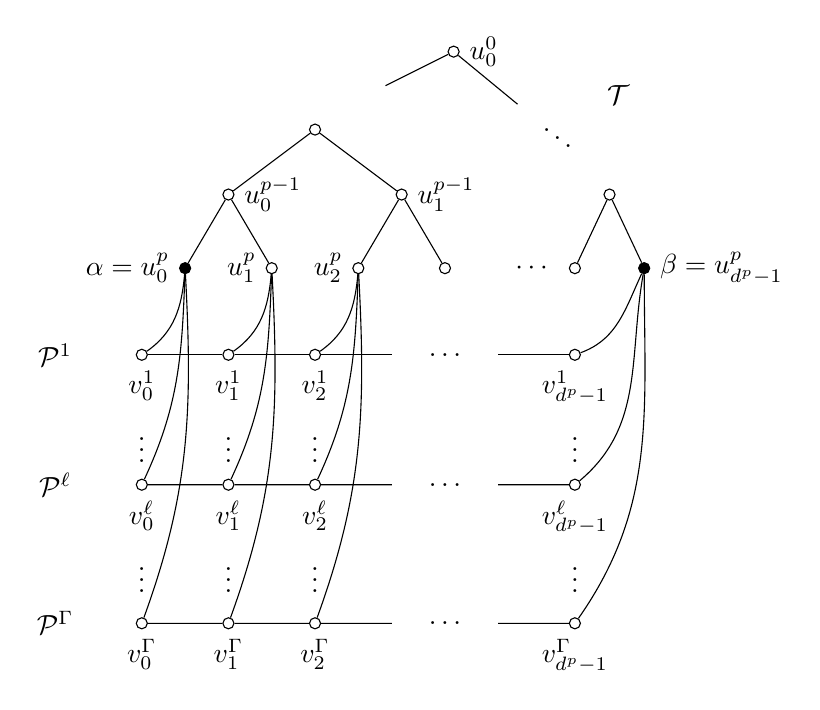
\begin{tikzpicture}[scale=1.1]
    % Define styles for different types of vertices
    \tikzset{
        vertex/.style={circle, draw, minimum size=4pt, inner sep=1pt, fill=white},
        filled/.style={circle, draw, fill=black, minimum size=4pt, inner sep=1pt},
    }
    
    
    % Draw vertices on level A with labels
    \node[] at (-1,0) {$\mathcal{P}^1$};
    \node[vertex] (a) at (0,0) [label=below:$v^1_0$] {};
    \node[vertex] (b) at (1,0) [label=below:$v^1_1$] {};
    \node[vertex] (c) at (2,0) [label=below:$v^1_2$] {};
    \node[] (ca) at (3,0) {};
    \node[] at (3.5,0) {$\dots$};
    \node[] (cb) at (4,0) {};
    \node[vertex] (d) at (5,0) [label=below:$v^1_{d^p-1}$] {};

    \node (dda) at (0,-1) {$\vdots$};
    \node (ddb) at (1,-1) {$\vdots$};
    \node (ddc) at (2,-1) {$\vdots$};
    \node (ddd) at (5,-1) {$\vdots$};
    \node (ddda) at (0,-2.5) {$\vdots$};
    \node (dddb) at (1,-2.5) {$\vdots$};
    \node (dddc) at (2,-2.5) {$\vdots$};
    \node (dddd) at (5,-2.5) {$\vdots$};
    
    % Draw vertices on level B with labels
    \node[] at (-1,-1.5) {$\mathcal{P}^\ell$};
    \node[vertex] (e) at (0,-1.5) [label=below:$v^\ell_0$] {};
    \node[vertex] (f) at (1,-1.5) [label=below:$v^\ell_1$] {};
    \node[vertex] (g) at (2,-1.5) [label=below:$v^\ell_2$] {};
    \node[] (ga) at (3,-1.5) {};
    \node[] at (3.5,-1.5) {$\dots$};
    \node[] (gb) at (4,-1.5) {};
    \node[vertex] (h) at (5,-1.5) [label=below:$v^\ell_{d^p-1}$] {};
    
    % Draw vertices on level C with labels
    \node[] at (-1,-3.1) {$\mathcal{P}^\Gamma$};
    \node[vertex] (i) at (0,-3.1) [label=below:$v^\Gamma_0$] {};
    \node[vertex] (j) at (1,-3.1) [label=below:$v^\Gamma_1$] {};
    \node[vertex] (k) at (2,-3.1) [label=below:$v^\Gamma_2$] {};
    \node[] (ka) at (3,-3.1) {};
    \node[] at (3.5,-3.1) {$\dots$};
    \node[] (kb) at (4,-3.1) {};
    \node[vertex] (l) at (5,-3.1) [label=below:$v^\Gamma_{d^p-1}$] {};
    
    % Draw tree structure vertices
    \node at (5.5,3) {$\mathcal{T}$};
    \node[vertex] (o) at (3.6,3.5) [label=right:$u_0^0$] {};
    
    \node (left) at (2.7,3.05) {};
    \node (right) at (4.45,2.8) {};
    
    \node (eleft) at (2.45,3) {$\iddots$};
    \node (eright) at (4.8,2.6) {$\ddots$};
    \node[vertex] (pq) at (2,2.6) {};
    
    \node[vertex] (p) at (1,1.85) [label=right:$u^{p-1}_0$] {};
    \node[vertex] (q) at (3,1.85) [label=right:$u^{p-1}_1$] {};
    \node[vertex] (qq) at (5.4,1.85) {};
    
    \node[filled] (s) at (0.5,1) [label=left:{$\alpha=u^p_0$}] {};
    \node[vertex] (m) at (1.5,1) [label=left:$u^p_1$] {};
    \node[vertex] (n) at (2.5,1) [label=left:$u^p_2$] {};
    \node[vertex] (nn) at (3.5,1) {};
    \node (mid) at (4.5,1) {$\cdots$};
    \node[vertex] (rl) at (5,1) {};
    \node[filled] (r) at (5.8,1) [label=right:{$\beta=u^p_{d^p-1}$}] {};
    
    % Draw path connections
    \draw (a) -- (b) -- (c) -- (ca);
    \draw (e) -- (f) -- (g) -- (ga);
    \draw (i) -- (j) -- (k) -- (ka);
    \draw (cb) -- (d);
    \draw (gb) -- (h);
    \draw (kb) -- (l);
    
    % Draw tree connections
    \draw (o) -- (left);
    \draw (o) -- (right);
    \draw (p) -- (pq);
    \draw (q) -- (pq);
    \draw (p) -- (s);
    \draw (p) -- (m);
    \draw (q) -- (n);
    \draw (q) -- (nn);
    \draw (qq) -- (r);
    \draw (qq) -- (rl);
    
    \draw (s) to [out=265, in=35] (a);
    \draw (s) to [out=268, in=65] (e);
    \draw (s) to [out=273, in=70] (i);
    \draw (m) to [out=265, in=35] (b);
    \draw (m) to [out=268, in=65] (f);
    \draw (m) to [out=273, in=70] (j);
    \draw (n) to [out=265, in=35] (c);
    \draw (n) to [out=268, in=65] (g);
    \draw (n) to [out=273, in=70] (k);
    \draw (r) to [out=245, in=20] (d);
    \draw (r) to [out=260, in=40] (h);
    \draw (r) to [out=270, in=55] (l);
\end{tikzpicture}
    \caption{An example of $\GGdp$ with $d=2$.}
    \label{fig:GGdp}
\end{figure}

We restate the simulation lemma of \citet{das2011distributed}, which connects the computation of Boolean function in the traditional communication complexity model to the computation of Boolean function in the distributed model in graph $\GGdp$ with input vertices $\alpha$ and $\beta$.


% \yanyu{maybe the lemma before the simulation lemma is also needed. (will add later if it's needed)}
\begin{lemma}[Simulation lemma \cite{das2011distributed}]
\label{thm:simulation}
For any $\Gamma$, $d$, $p$, $B$, $\epsilon\geq 0$, and function $f:\bin^b \times \bin^b \to \bin$, if there is an $\epsilon$-error randomized distributed algorithm that computes $f(x,y)$ faster than $\frac{d^p-1}{2}$ rounds on $\GGdp$ with $x$ given to vertex $\alpha$ and $y$ given to vertex $\beta$, i.e.,
$
R_\epsilon^{\GGdp}(f) < \frac{d^p-1}{2},
$
then there is an $\epsilon$-error randomized algorithm in the communication complexity model that computes $f$ using at most $2dpB R_\epsilon^{\GGdp}(f)$ bits of communication.
In other words,
$
R_\epsilon^{cc-pub}(f)\leq 2dpB R_\epsilon^{\GGdp}(f).
$
% \yijun{When I first read the theorem I found it very confusing. I think an important point that is missing is that you need to say how the input to the function $f$ is stored in the network.}
\end{lemma}
%\yijun{rounds in distributes setting, bits in communication complexity}

% The simulation lemma was proved by carefully analyzing the states of the distributed (sub)-network over rounds, and showing that only $O(dp)$ messages are needed for Alice and Bob to simulate one round of the execution of any distributed algorithm on $\GGdp$. Hence, Alice and Bob can perform the above simulation and run any distributed algorithm for computing functions on $\alpha$ and $\beta$ on $\GGdp$ in the communication complexity model with only $O(dp)$-factor overhead.

% \yijun{Some suggestions: 
% (1) Include a very brief proof idea for the simulation lemma. 
% (2) Include a very brief proof sketch (no theorems, just a paragraph) for how the simulation lemma is used to give $\Omega(\sqrt{n})$ for one problem. Otherwise, the reader might be very lost.
% }
% \yanyu{(1) above (2) below}
The simulation lemma was proved by analyzing the states of the distributed (sub)-network over rounds. In $\GGdp$, Alice and Bob have two ways to communicate $b$ bits: either through paths of length $d^p-1$ between them, or through the tree structure. When an algorithm's runtime is less than $(d^p-1)/2$, messages cannot traverse the full path between Alice and Bob, forcing communication through the tree structure. This creates a congestion bottleneck which is manifested by their analysis that only $O(dp)$ messages are needed to simulate all messages sent in each round of the distributed algorithm on $\GGdp$. This allows Alice and Bob to simulate any distributed algorithm for computing functions $f$ on $\alpha$ and $\beta$ on $\GGdp$ in the communication complexity model with an $O(dp)$-factor overhead.
%\yanyu{edited}
%\yijun{the paragraph above essentially conveys zero information... I would at least explain why the threshold $(d^p-1)/2$ makes sense: Essentially there are two ways for Alice and Bob to communicate $\Theta(d^p)$ bits of information to each other: via paths or via trees, the first suffers from a dilation of $\Theta(d^p)$, the second suffers from a congestion of $\Theta(d^p)$}

The main way the above simulation lemma is used is via the following lemma which applies the simulation lemma specifically for the $\disj$ function. It translates the lower bound for $\disj$ in the communication model to a lower bound for computing $\disj$ in $\GGdp$ on $\alpha$ and $\beta$. 

\begin{lemma}[Set disjointness lower bound for $\GGdp$~\cite{das2011distributed}]\label{lem:disj}
For any $\Gamma, d, p$, there exists a constant $\epsilon>0$ such that
$$R_\epsilon^{\GGdp}\left(\disj_b;B\right)=\Omega\left(\min\left(d^p, \frac{b}{dpB}\right)\right).$$
\end{lemma}






\subsection{Modification to \GGdptitle{}}
\label{subsec:modification}

In this section, we present our graph construction $\Gkdpp$ builds upon $\GGdp$ to allow us to perform a reduction from distributed set disjointness to the \secsisp{} and \rpath{} problems. Compared with the $\widetilde{\Omega}(\sqrt{n})$ lower bounds obtained via existing constructions~\cite{das2011distributed,manoharan2024computing}, our graph construction $\Gkdpp$ allows us to obtain a higher $\widetilde{\Omega}(n^{2/3})$ lower bound. 
%\yijun{the first sentence is a bit awkward}
We show how to simulate any distributed disjointness algorithm for $\Gkdpp$ on $\GGdp$ with $O(1)$-factor overhead. Connecting these two results, we obtain a lower bound for computing disjointness on $\Gkdpp$ with inputs given to $\alpha$ and $\beta$.

\paragraph{Intuition.} Our lower bound construction is built around a bipartite graph positioned at the far end of the structure, which controls the replacement path distances for each edge along the given $s$-$t$ path. We aim to establish a correspondence between the edge orientations in the bipartite graph and the replacement path distances for the edges in the given $s$-$t$ path. Moreover, we require that reversing the orientation of the edges in the bipartite graph result in longer replacement paths. To solve the replacement path problem, Alice must learn the orientation of every edge in the bipartite graph, requiring substantial information to be transmitted from one end to the other.
%\yanyu{edited}
% so that the length of the second simple shortest path, i.e. the minimum replacement path across all edges in the given $s$-$t$ path, can be used to indicate the disjointness between two parties. 
% \yanyu{is this confusing out of context?}
% \yijun{This is confusing because You only discuss $M$ and omit $x$ entirely. There are two ways to improve the writing: One is that here you just say that to solve replacement paths we need to learn all the edge orientations in the bipartite graphs (without mentioning \secsisp{} and set disjointness), requiring transmitting a lot of information from one end to the other end. Second is to include more detail of not only $M$ but also $x$ and say that they correspond to the set disjointness input and how they affect replacement path length (you can also choose to do this later in the place where you introduce them).}

The construction proceeds by first establishing a mapping between each edge on the $s$-$t$ path and its corresponding edge in the bipartite graph. 
For each edge in the $s$-$t$ path, we connect a long path to its mapped edge in the bipartite graph.
% to increase the distance between the given $s$-$t$ path and the bipartite graph where the direction information is stored. 
The long distance between the output vertices (vertices in the given $s$-$t$ path) and the location of critical information (edge orientations in the bipartite graph) forces the algorithm to spend more rounds propagating information to their required destinations. 
The orientation of the edges in the bipartite graph determines the length of the replacement path for their corresponding edges. %This correspondence is critical for computing disjointness. 
With $n^{1/3}$ paths of length approximately $n^{2/3}$, the algorithm requires at least $n^{2/3}$ rounds to propagate this critical information. 
Next, to reduce the graph's diameter without creating additional replacement paths, we incorporate a tree-like structure with downward edge orientations along the path. As demonstrated in the simulation lemma of \citet{das2011distributed} and our new simulation in \Cref{lem:disj G(kdpp)}, this structure does not substantially improve the propagation of critical information.
Finally, to optimize the total number of vertices, we carefully merge paths that lead to the same vertex in the bipartite graph while ensuring that the correspondence between edge orientations in the bipartite graph and replacement path lengths remains intact.
%\yanyu{edited}
% \yijun{I did not see the main idea being explicitly mentioned: the orientation of each edge in the bipartite graph controls the replacement path length for the corresponding edge (for one direction, you can use that in the replacement path, for the other direction, you need to take a longer detour), so the replacement path distance can be used to determine the direction of the corresponding edge in the bipartite graph. Therefore, solving the replacement path problem requires communicating $\Omega(n^{2/3})$ bits of information from one side of the graph to the other side of the graph.}


\paragraph{Construction of \Gkdpptitle.}
Our modified graph is called $\Gkdpp$ where $\phi: [k^2] \to [k]\times[k]$ is a bijection used to map any edge $\left(s_{i-1}, s_i\right)$ on the given $s$-$t$ path to an edge on the bipartite graph. Refer to \Cref{fig:Gkdpp} for an illustration. We present the construction of $\Gkdpp$ with some default edge orientation. %If the problem in consideration only concerns undirected graph, then ignore the default direction provided. [Yi-Jun: I commented out the above sentence as it seems irrelevant to us]
The graph $\Gkdpp$ is constructed via the following steps:
% \yijun{
% This is a complicated construction. Need to give intuition. Also, 
% try to give a proof sketch/idea before presenting the formal proofs in the next sub-section.}
\begin{enumerate}
    \item Construct $\GGdp$ with $\Gamma = 2k$. We relabel the vertices of the last $k$ paths by $w^\ell_i$, where $1\leq\ell\leq k$ and $0\leq i\leq d^p-1$. For $1\leq\ell\leq k$, we use the shorthand $v^\ell$ and $w^\ell$ to denote the \emph{last} vertex of path $\Pc^\ell$ and $\Pc^{\ell+k}$, respectively. 
    \item For $1\leq i,j \leq k$, add edges $\{v^i, w^j\}$.
    \item Add a directed path $\mathcal{P^*}$ with $k^2$ edges from $s$ to $t$.\\ We label the vertices on the path by $s=s_0, s_1, \dots, s_{k^2}=t$. 
    \item Add $k$ paths $\Qc^1, \dots, \Qc^k$ each of length $2k^2$, where $\Qc^\ell$ consists of vertices $q^\ell_0, \dots, q^\ell_{2k^2}$. \\For each $1\leq\ell\leq k$, add edge $\left(q^{\ell}_{2k^2}, v^{\ell}_0\right)$.
    \item Add $k$ paths $\Rc^1, \dots, \Rc^k$ each of length $2k^2$, where $\Rc^\ell$ consists of vertices $r^\ell_0, \dots, r^\ell_{2k^2}$. \\For each $1\leq\ell\leq k$, add edge $\left(w^{\ell}_0, r^{\ell}_{0}\right)$.
    \item For $i\in [k^2]$, suppose $\phi(i)=\left(\phi_1(i),\phi_2(i)\right)$, add $\left\{s_{i-1}, q^{\phi_1(i)}_{2(i-1)}\right\}$ and $\left(r^{\phi_2(i)}_{2i}, s_i\right)$.
    \item Add edges from $\alpha$ to all vertices in $\Pstar, \Qc^i, \Rc^i$, for each $1\leq i \leq k$.
\end{enumerate}

\paragraph{Direction of edges.}
To facilitate our reduction from set disjointness to \secsisp{}, we assigned default orientations for all edges in $\Gkdpp$ except for those in the right bipartite graph and edges of the form $\left\{s_{i-1}, q^{\phi_1(i)}_{2(i-1)}\right\}$. The direction of the edges on the bipartite graph is determined by a matrix $M\in \bin^{k\times k}$ and the direction of the edges $\left\{s_{i-1}, q^{\phi_1(i)}_{2(i-1)}\right\}$ are determined by a vector $x\in \bin^{k^2}$. The directed version of the graph $\GkdppMx$ is constructed as follows.

\begin{enumerate}
    \item Orient the edges in paths $\Pstar, \Pc^\ell, \Qc^\ell, \Rc^\ell$ pointing to larger index for $1\leq \ell \leq k$ and orient the edges in paths $\Pc^\ell$ pointing to smaller index for $k+1\leq \ell \leq 2k$.
    \item Orient the edges in the tree $\Tc$ from parents to children. Orient the edges between the leaves and the paths pointing away from the leaves.  
    \item For $1\leq i,j \leq k$, add edge $(v^i, w^j)$ if $M_{ij}=1$. Otherwise, add edge $(w^j, v^i)$.
    \item For $i\in [k^2]$, set direction as $\left(s_{i-1}, q^{\phi_1(i)}_{2(i-1)}\right)$ if $x_i = 1$. Otherwise, set direction as $\left(q^{\phi_1(i)}_{2(i-1)}, s_{i-1}\right)$.
\end{enumerate}

When $x_i = 1$, alternative paths avoiding $\left(s_{i-1}, s_i\right)$ can use the edge $\left(s_{i-1}, q^{\phi_1(i)}_{2(i-1)}\right)$ to make a detour. Conversely, when $x_i = 0$, any alternative paths avoiding $(s_{i-1}, s_i)$ must leave $\Pstar$ before $s_{i-1}$. Since the paths $\Qc^\ell$ have double the length, alternative paths exiting earlier will have longer lengths. If the corresponding edge in the bipartite graph is oriented as $\left(v^{\phi_1(i)}, w^{\phi_2(i)}\right)$ (i.e. when $M_{\phi_1(i), \phi_2(i)}=1$), the returning detour using the edge $\left(r^{\phi_2(i)}_{2i}, s_i\right)$ can be taken. For the same reason, detours returning earlier will have shorter lengths. Hence, the shortest detour is possible if and only if both $x_i = 1$ and $M_{\phi_1(i), \phi_2(i)}=1$, allowing us to reduce set disjointness to \secsisp{}.

%\yanyu{added motivation behind $M$ and $x$}
% \yijun{Now is the right place to explain the motivation behind $M$ and $x$: Say that they correspond to the set disjointness input, and intuitively how their values affect replacement path length.}
% Firstly, we consider $\Gamma = 2k$ and we relabel the vertices of the last $k$ path as $w^\ell_i$. Now, we add a directed path $\mathcal{P^*}$ with $k^2$ edges from $s$ to $t$. We label the vertices on the path by $s=s_0, s_1, \dots, t=s_{k^2}$. 
% Then consider a bijection $\phi: [k^2] \to [k]\times[k]$. Suppose $\phi(i) = (\phi(i)_1, \phi(i)_2)$, this bijection is used to map any edge $\left(s_{i-1}, s_i\right)$ on $\Pstar$ to a vertex pair $\left(v^{\phi(i)_1}, w^{\phi(i)_2}\right)$. 
% Then we further add $2k$ number of paths $\Qc^1, \dots, \Qc^k$ and $\Rc^1, \dots, \Rc^k$, each having $2k^2$ edges, with vertices indexed from $0$ to $2k^2$. For each $1\leq\ell\leq k$, add edges $\left(q^{\ell}_{2k^2}, v^{\ell}_0\right)$ and $\left(w^{\ell}_0, r^{\ell}_{0}\right)$
% For each edge $(s_{i-1}, s_i)$, add $\left(s_{i-1}, q^{\phi(i)_1}_{2(i-1)}\right)$ and $\left(r^{\phi(i)_2}_{2i}, s_i\right)$. Lastly, we add edges from $\alpha$ to all vertices on $\Pstar, \Qc^i, \Rc^i$.


\begin{figure}[ht!]
    \centering
    \begin{tikzpicture}[scale=1.1]
\scriptsize
    % Define styles for different types of vertices
    \tikzset{
        vertex/.style={circle, draw, minimum size=4pt, inner sep=1pt, fill=white},
        filled/.style={circle, draw, fill=black, minimum size=4pt, inner sep=1pt},
        symbol/.style={inner sep=0pt, font=\small, text height=12pt},
        small/.style={font=\small},
        mapping/.style={teal!60!blue, thick},
        dir/.style={arrows = {-Stealth[inset=0.7pt, length=5pt, angle'=25]}},
        widedir/.style={arrows = {-Stealth[inset=0.7pt, length=5pt, angle'=35]}},
        highlight/.style={teal!70!green, thick},
        hlar/.style={highlight, dir},
        line/.style={gray, very thin, dir},
    }
    
    % Draw vertices on level A with labels
    \node[] at (-0.4,0) {$\mathcal{P}^1$};
    \node[vertex] (a) at (0,0) [label=below:$v^1_0$] {};
    \node[vertex] (b) at (1,0) [label=below:$v^1_1$] {};
    \node[vertex] (c) at (2,0) [label=below:$v^1_2$] {};
    \node[] (ca) at (3.5,0) {};
    % \node[] (ca2) at (3.5,0) {};
    \node[small] at (4,0) {$\cdots$};
    \node[] (cb) at (4.5,0) {};
    \node[vertex] (d) at (7.5,0) [label=right:{$v^1=v^1_{d^p-1}$}] {};

    \node[symbol] (dda) at (0,-0.7) {$\vdots$};
    \node[symbol] (ddb) at (1,-0.7) {$\vdots$};
    \node[symbol] (ddc) at (2,-0.7) {$\vdots$};
    \node[symbol] (ddd) at (6.6,-0.6) {$\iddots$};
    
    \node[symbol] (ddda) at (0,-3.8) {$\vdots$};
    \node[symbol] (dddb) at (1,-3.8) {$\vdots$};
    \node[symbol] (dddc) at (2,-3.8) {$\vdots$};
    \node[symbol] (dddd) at (6.6,-3.4) {$\ddots$};
    
    % Draw vertices on level B with labels
    \node[] at (-0.4,-1.2) {$\mathcal{P}^k$};
    \node[vertex] (e) at (0,-1.2) [label=below:$v^k_0$] {};
    \node[vertex] (f) at (1,-1.2) [label=below:$v^k_1$] {};
    \node[vertex] (g) at (2,-1.2) [label=below:$v^k_2$] {};
    \node[] (ga) at (3.5,-1.2) {};
    \node[small] at (4,-1.2) {$\cdots$};
    \node[] (gb) at (4.5,-1.2) {};
    \node[vertex] (h) at (6,-1.2) [label=below left:{$v^k$}] {};

    % Draw vertices on level C with labels
    \node[] at (-0.5,-2.8) {$\mathcal{P}^{k+1}$};
    \node[vertex] (e2) at (0,-3) [label=below:$w^1_0$] {};
    \node[vertex] (f2) at (1,-3) [label=below:$w^1_1$] {};
    \node[vertex] (g2) at (2,-3) [label=below:$w^1_2$] {};
    \node[] (ga2) at (3.5,-3) {};
    \node[small] at (4,-3) {$\cdots$};
    \node[] (gb2) at (4.5,-3) {};
    \node[vertex] (h2) at (6,-3) [label=below:{$w^1$}] {};
    
    
    % Draw vertices on level D with labels
    \node[] at (-0.5,-4) {$\mathcal{P}^{2k}$};
    \node[vertex] (i) at (0,-4.2) [label=below:$w^k_0$] {};
    \node[vertex] (j) at (1,-4.2) [label=below:$w^k_1$] {};
    \node[vertex] (k) at (2,-4.2) [label=below:$w^k_2$] {};
    \node[] (ka) at (3.5,-4.2) {};
    \node[small] at (4, -4.2) {$\cdots$};
    \node[] (kb) at (4.5,-4.2) {};
    \node[vertex] (l) at (7.5,-4.2) [label=below:{$w^k=w^k_{d^p-1}$}] {};
    
    % Draw tree structure vertices
    \begin{scope}[xshift=1.5mm, yshift=0mm]
        \node at (5,3) {$\mathcal{T}$};
        \node[vertex] (o) at (3.3,3.6) [label=right:$u_0^0$] {};
        
        \node (left) at (2.7,3.2) {};
        \node (right) at (4.1,3.0) {};
        
        \node[symbol] (eleft) at (2.4,3.1) {$\iddots$};
        \node[symbol] (eright) at (4.5,2.7) {$\ddots$};
        \node[small] (mid) at (4,1) {$\cdots$};
        \node[vertex] (pq) at (2,2.8) {};
        
        \node[vertex] (p) at (1,2) [label=right:$u^{p-1}_0$] {};
        \node[vertex] (q) at (2.9,2) [label=right:$u^{p-1}_1$] {};
        \node[vertex] (qq) at (5.1,2) {};
        
        \node[filled] (s) at (0.5,) [label=above left:{$\alpha=u^p_0$}] {};
        \node[vertex] (m) at (1.5,1) [label=left:$u^p_1$] {};
        \node[vertex] (n) at (2.5,1) [label=left:$u^p_2$] {};
        \node[vertex] (nn) at (3.3,1) {};
        \node[vertex] (rl) at (4.7,1) {};
        \node[filled] (r) at (5.5,1) [label=above right:{$\beta=u^p_{d^p-1}$}] {};
    \end{scope}
    % Draw path connections
    \draw[dir, highlight] (a) -- (b) -- (c) -- (ca);
    \draw[dir] (e) -- (f) -- (g) -- (ga);
    \draw[dir] (ga2) -- (g2) -- (f2) -- (e2);
    \draw[dir, highlight] (ka) -- (k) -- (j) -- (i);
    \draw[dir, highlight] (cb) -- (d);
    \draw[dir] (gb) -- (h);
    \draw[dir] (h2) -- (gb2);
    \draw[dir, highlight] (l) -- (kb);
    
    % Draw tree connections
    \draw[line] (o) -- (left);
    \draw[line] (o) -- (right);
    \draw[line] (pq) -- (p);
    \draw[line] (pq) -- (q);
    \draw[line] (p) -- (s);
    \draw[line] (p) -- (m);
    \draw[line] (q) -- (n);
    \draw[line] (q) -- (nn);
    \draw[line] (qq) -- (r);
    \draw[line] (qq) -- (rl);
    
    \draw[line] (s) to [out=269,in=35] (a);
    \draw[line] (s) to [out=269,in=50] (e);
    \draw[line] (s) to [out=272,in=60] (e2);
    \draw[line] (s) to [out=275,in=60] (i);
    
    \draw[line] (m) to [out=269,in=35] (b);
    \draw[line] (m) to [out=269,in=50] (f);
    \draw[line] (m) to [out=272,in=60] (f2);
    \draw[line] (m) to [out=275,in=60] (j);
    
    \draw[line] (n) to [out=268,in=35] (c);
    \draw[line] (n) to [out=269,in=50] (g);
    \draw[line] (n) to [out=272,in=60] (g2);
    \draw[line] (n) to [out=275,in=60] (k);
    
    \draw[line] (r) to [out=355,in=115] (d);
    \draw[line] (r) to [out=300,in=85] (h);
    \draw[line] (r) to [out=260,in=120, looseness=1] (h2);
    \draw[line] (r) to [out=258,in=175, looseness=1.2] (l);

    % Bipartite graph mapped from the string y
    \node (vl) at (6.95,-0.25) {};
    \node (wl) at (6.95,-3.85) {};
    \draw[dir, mapping] (d) -- (h2);
    \draw[dir, mapping] (d) -- (wl);
    \draw[dir, mapping] (vl) -- (l);
    \draw[dir, mapping] (wl) -- (vl);
    \draw[dir, mapping] (vl) -- (h2);
    \draw[dir, mapping] (h) -- (l);
    \draw[dir, mapping] (h2) -- (h);
    \draw[dir, mapping] (wl) -- (h);
    \draw[widedir, highlight, very thick] (d) -- (l);

    \begin{scope}[xshift=-35mm, yshift=-1mm]
        \node[vertex] (s0) at (0,-4) [label=left:{$s=s_0$}] {};
        \node[vertex] (s1) at (0,-3) [label=left:$s_1$] {};
        \node[symbol] (s2) at (0,-2) {$\vdots$};
        \node[vertex] (sj) at (0,-1) [label=below left:$s_{i-1}$] {};
        \node[vertex] (si) at (0,0) [label=below left:$s_i$] {};
        \node[symbol] (s5) at (0,1) {$\vdots$};
        \node[vertex] (st) at (0,2) [label=below left:{$t=s_{k^2}$}] {};
        \node[symbol] (Pstar) at (-0.1,2.52)  {$\mathcal{P}^*$};

        \draw[dir, highlight] (s0) -- (s1);
        \draw[dir, highlight] (s1) -- (s2);
        \draw[dir, highlight] (s2) -- (sj);
        \draw[dir, red, thick] (sj) -- (si);
        \draw[dir, highlight] (si) -- (s5);
        \draw[dir, highlight] (s5) -- (st);

        \node[symbol] (Q)  at (1.2,2.5)    {$\mathcal{Q}^1$};
        \node[vertex] (q0)  at (1.3,-4)     [label=right:{$q^1_0$}] {};
        \node[vertex] (q05) at (1.3,-3.5) [label=right:{$q^1_1$}] {};
        \node[vertex] (q1)  at (1.3,-3)    [label=right:{$q^1_2$}] {};
        \node[symbol] (q2)  at (1.3,-2) {$\vdots$};
        \node[vertex] (qj)  at (1.3,-1)    [label=below right:$q^1_{2i-2}$]{};
        \node[vertex] (qji) at (1.3,-0.5) [label=right:$q^1_{2i-1}$]{};
        \node[vertex] (qi)  at (1.3,0)     [label=right:$q^1_{2i}$] {};
        \node[symbol] (q5)  at (1.3,1) {$\vdots$};
        \node[vertex] (qt)  at (1.3,2)     [label=below right:{$q^1_{2k^2}$}] {};

        \draw[dir] (q0)  -- (q05);
        \draw[dir] (q05) -- (q1);
        \draw[dir] (q1)  -- (q2);
        \draw[dir] (q2)  -- (qj);
        \draw[dir, highlight] (qj)  -- (qji);
        \draw[dir, highlight] (qji) -- (qi);
        \draw[dir, highlight] (qi)  -- (q5);
        \draw[dir, highlight] (q5)  -- (qt);

        \node[symbol] (r)  at (-1.5,2.55)    {$\mathcal{R}^k$};
        \node[vertex] (r0)  at (-1.5,-4)    [label=left:{$r^k_0$}] {};
        \node[vertex] (r05) at (-1.5,-3.5)  [label=left:{$r^k_1$}] {};
        \node[vertex] (r1)  at (-1.5,-3)    [label=left:{$r^k_2$}] {};
        \node[symbol] (r2)  at (-1.5,-2) {$\vdots$};
        \node[vertex] (rj)  at (-1.5,-1)    [label=left:$r^k_{2i-2}$]{};
        \node[vertex] (rji) at (-1.5,-0.5)  [label=left:$r^k_{2i-1}$]{};
        \node[vertex] (ri)  at (-1.5,0)     [label=above left:$r^k_{2i}$] {};
        \node[symbol] (r5)  at (-1.5,1) {$\vdots$};
        \node[vertex] (rt)  at (-1.5,2)     [label=below left:{$r^k_{2k^2}$}] {};

        \draw[dir, highlight] (r0)  -- (r05);
        \draw[dir, highlight] (r05) -- (r1);
        \draw[dir, highlight] (r1)  -- (r2);
        \draw[dir, highlight] (r2)  -- (rj);
        \draw[dir, highlight] (rj)  -- (rji);
        \draw[dir, highlight] (rji) -- (ri);
        \draw[dir] (ri)  -- (r5);
        \draw[dir] (r5)  -- (rt);
        
        \draw[hlar] (ri)  to [out=20,in=165] (si);
        \draw[hlar] (sj)  to [out=345,in=200] (qj);
    \end{scope}

    \draw[dir, highlight] (qt)  to [out=30,in=120] (a);
    \draw[dir, highlight] (i)  to [out=200,in=320] (r0);
    \node[symbol] (PPP)  at (-1.5,-5) {{\color{teal!70!green}$P$}};
\end{tikzpicture}
    \caption{Illustration of $\Gkdpp$, assuming $\phi(i)=(1,k)$ and $M_{1,k} = 1$. Paths $\Qc^2,\dots,\Qc^k$ and $\Rc^1,\dots,\Rc^{k-1}$ are omitted. Other edges from $\Pstar$ to $\Qc^1$, and from $\Rc^k$ to $\Pstar$ are omitted. Edges from $\alpha$ to $\Pstar, \Qc^i$ and $\Rc^i$ are omitted. Reversed directional edges in the bipartite graph are omitted. When $(v^1, w^k)$ is oriented correctly, the green highlighted path $P$ is a replacement path from $s$ to $t$ for the deleted edge $(s_{i-1}, s_i)$.}
    \label{fig:Gkdpp}
\end{figure}

\begin{observation}[Basic properties of $\Gkdpp$]\label{obs:Gkdpp}
    There are $\Theta(k^3 + k d^p)$ vertices in $\Gkdpp$, and the diameter of $\Gkdpp$ is at most $2p+2$.
\end{observation}
    % \yijun{add a very short proof: especially the diameter part.}

\begin{proof}
    The number of vertices for the respective parts are: $2k d^p$ vertices for $\Pc^\ell$, $2k \times (2k^2+1)$ for $\Rc^\ell$ and $\Qc^\ell$, $k^2+1$ vertices for $\Pstar$ and $\frac{d^{p+1}-1}{d-1}$ vertices for $\Tc$. Hence the total number of vertices is $2k d^p +4k^3 + 2k + k^2 + 1 + \frac{d^{p+1}-1}{d-1} = \Theta(k^3+kd^p)$. Every vertex not on the tree $\Tc$ is connected to some leaf in $\Tc$. Since $\Tc$ has depth $p$, the diameter of $\Gkdpp$ is at most $2p+2$.
\end{proof}
    
Now we show a lemma for a lower bound of distributed algorithms for set disjointness on $\Gkdpp$. This is analogous to \Cref{lem:disj}. We achieve this by applying \Cref{thm:simulation} and \Cref{lem:disj} in a black-box manner, and showing how distributed algorithms for set disjointness on $\Gkdpp$ can be simulated on $\GGdp$ with $O(1)$-factor overhead. The intuition for the simulation is that $\alpha$ will simulate the vertices in $\Pstar, \Qc^\ell$ and $\Rc^\ell$ and $\beta$ will simulate the vertices in the bipartite graph. 


% \begin{theorem}[simulation lemma II]
% \label{thm:simulation G(kdpp)}
% For any $k$, $d$, $p$, $B$, bijection $\phi: [k^2]\to [k]\times [k]$ and matrix $M \in \bin^{k\times k}$,
% any $T$-round distributed algorithm $\Ac$ on $\Gkdpp$ can be simulated in $\GGdp$, with $\Gamma=2k$ in $3T$ rounds.
% \end{theorem}
% \yanyu{do we need to say what do we mean by ``simulate'' or is it clear in this context?}
% \yijun{I think you can avoid this issue by removing this theorem and incorporating the proof into the lemma below.}


% \begin{proof}
    
% \end{proof}


\begin{lemma}[Set disjointness lower bound for $\Gkdpp$]
\label{lem:disj G(kdpp)}
    For any $k, d, p$ and bijection $\phi: [k^2]\to [k]\times [k]$ there exists a constant $\epsilon>0$ such that
    $$R_\epsilon^{\Gkdpp}\left(\disj_b;B\right)=\Omega\left(\min\left(d^p, \frac{b}{dpB}\right)\right).$$
\end{lemma}

\begin{proof}
    First, we show that if there is a $T$-round distributed algorithm for set disjointness $\Ac$ on $\Gkdpp$, then there is a $3T$-round distributed algorithm for set disjointness on $\GGdp$. We achieve this via simulating $\Ac$ on $\GGdp$.

    Suppose we have an algorithm $\Ac$ on graph $\GkdppMx$, we will denote a message sent in the $i$th round of $\Ac$ from vertex $u$ to vertex $v$ as $\Mc_i(u\to v)$. 
    Now $\alpha$ in $\GGdp$ can simulate all the vertices in $\Rc^\ell, \Qc^\ell$ and $\Pstar$ in the following way. 
    vertex $\alpha$ will run $2k+2$ processes and run $\Ac$ for $\alpha, \Rc^\ell, \Qc^\ell$ and $\Pstar$ for $1\leq \ell \leq k$ on these processes. 
    Any messages among the vertices in $\alpha, \Rc^\ell, \Qc^\ell$ and $\Pstar$ can be handled locally between the processes.
    The only messages left are between $v^\ell_0$ and $q^\ell_{2k^2}$ and between $w^\ell_0$ and $r^\ell_0$, where $1\leq \ell\leq k$. For each $1\leq \ell\leq k$, $\Mc_i(q^\ell_{2k^2}\to v^\ell_0)$ and $\Mc_i(v^\ell_0 \to q^\ell_{2k^2})$ are delivered along the edge $\{q^\ell_{2k^2}, v^\ell_0\}$. Similarly, $\Mc_i(r^\ell_{0}\to w^\ell_0)$ and $\Mc_i(w^\ell_0 \to r^\ell_{0})$ are delivered along the edge $\{r^\ell_{0}, w^\ell_0\}$.  
    Since there are at most twice the number of messages along the edges of $\alpha$, we can simulate $\Ac$ on $\GGdp$ in $3T$ rounds.

    Now we describe how to handle the bipartite graph in $\GkdppMx$ in vertex $\beta$ on $\GGdp$. vertex $\beta$ will create $2k+1$ processes that run $\Ac$ acting as $\beta, v^\ell$ and $w^\ell$ locally, where $1\leq \ell\leq k$. Any messages among these vertices are handled locally on $\beta$. The only messages left are between $v^\ell_{d^p-2}$ and $v^\ell$ and between $w^\ell_{d^p-2}$ and $w^\ell$. We will focus on $v^\ell$ now since the behaviors on $w^\ell$ are similar. In the $(3i-2)$th round, vertex $v^\ell_{d^p-2}$ and $v^\ell$ exchange $\Mc_i(v^\ell_{d^p-2}\to v^\ell)$ and $\Mc_i(v^\ell\to v^\ell_{d^p-2})$. In the $(3i-1)$th round, $v^\ell$ relay $\Mc_i(v^\ell_{d^p-2}\to v^\ell)$ to $\beta$. $\beta$ now has all the information needed to compute $\Mc_{i+1}(v^\ell \to v^\ell_{d^p-2})$ locally. $\beta$ computes $\Mc_{i+1}(v^\ell \to v^\ell_{d^p-2})$ and send it to $v^\ell$ in the $3i$th round. Now $v^\ell$ has $\Mc_{i+1}(v^\ell \to v^\ell_{d^p-2})$ to send to $v^\ell_{d^p-2}$ in the $(3(i+1)-2)$th round and the process repeats.

    All other vertices in $\GGdp$ will execute their part of $\Ac$ with $2$ empty rounds between any two rounds in $\Ac$ to align their pace with that of vertices $\alpha$ and $\beta$.
    In this way, we can simulate any $T$-round algorithm on $\GkdppMx$ with $3T$ rounds on $\GGdp$.
    
    After applying \Cref{lem:disj}, we have the desired lower bound.
\end{proof}


\subsection{Lower Bound for the \secsisp{} Problem}
\label{subsec:lower bound reduction}
%\yijun{Shorten title name}
Now we are ready to show our main results: lower bounds for the \secsisp{} problem and the \rpath{} problem. We will show \Cref{thm:2sisp lower} by a reduction from the disjointness problem on $\Gkdpp$.
Before we show a reduction from disjointness to \secsisp{}, we show a correspondence between the replacement path lengths and the edge orientations in the bipartite graph.

\begin{lemma}[Replacement path lengths]
\label{lem:GkdppMx Rpath-dir correspondence}
    Consider the graph $\GkdppMx$. For any edge $(s_{i-1},s_i)$ in the path $\Pstar$, if $M_{\phi_1(i), \phi_2(i)}=1$ and $x_i=1$, the length of the replacement path is $3k^2 + 2 d^p + 6$. Otherwise, the length is strictly greater.
\end{lemma}

\begin{proof}
    Suppose $M_{\phi_1(i), \phi_2(i)}=1$ and $x_i = 1$, then the highlighted path $P$ as shown in \Cref{fig:Gkdpp} is an alternative path. It can be easily checked that it has length $3k^2 + 2 d^p + 6$. Now we show that it is the shortest among all alternative $s$-$t$ path. Observe that all alternative $s$-$t$ path must be of the form 
    $$s, \dots, s_{j-1}, q^{\phi_1(j)}_{2j-2}, \dots, q^{\phi_1(j)}_{2k^2}, \;\Pc^{\phi_1(j)},\; \Pc^{\phi_2(l)+k}, \;r^{\phi_2(l)}_0, \dots, r^{\phi_2(l)}_{2l}, s_l,\dots, t$$ where $j\leq i$ and $l\geq i$. 
    Notice that the length of the above path is $3k^2 + 2d^p + 4 + 2(l-j+1)$. This length is minimized when $l=j=i$ and we have our highlight path $P$ with length $3k^2 + 2 d^p + 6$.

    Conversely, suppose $M_{\phi_1(i), \phi_2(i)}=0$ or $x_i=0$. If $M_{\phi_1(i), \phi_2(i)}=0$, the shortest alternative path is has length greater than $3k^2 + 2 d^p + 6$. This is because, the choice of $j=l=i$ does not constitute a directed path anymore as the bipartite edge is oriented from $w^{\phi_2(i)}$ to $v^{\phi_1(i)}$. If $x_i=0$, then the alternate $s$-$t$ path must exit $\Pstar$ before $s_{i-1}$ and therefore has length greater than $3k^2 + 2 d^p + 6$.
\end{proof}

% \yijun{I think the proof of the lemma below is ok now (up to some minor typos).}
\begin{lemma}[Reducing set disjointness to \secsisp{}]\label{lem:Disj to 2sisp}
    For any $k$, $d\geq 2$, $p$, bijection $\phi: [k^2]\to [k]\times [k]$ and $\epsilon\geq 0$, if there exists an $\epsilon$-error randomized distributed algorithm for the \secsisp{} problem on graph $\GkdppMx$ for any $M\in \bin^{k\times k}$ and any $x\in \bin^{k^2}$ then there exists an $\epsilon$-error randomized algorithm for computing $\disj_{k^2}(x,y)$ (on $k^2$-bit inputs) on $\Gkdpp$ that uses the same round complexity with additional $O(\frac{k}{B})$ rounds.
\end{lemma}

\begin{proof}
    Suppose $\Ac$ is an $\epsilon$-error randomized distributed algorithm for the \secsisp{} problem and suppose we are given a set disjointness instance with $k^2$-bit strings on $\Gkdpp$. We aim to use $\Ac$ to solve the set disjointness problem $\disj_{k^2}(x,y)$.

    Suppose Alice received $x\in \bin^{k^2}$ on vertex $\alpha$ and Bob received $y\in \bin^{k^2}$ on vertex $\beta$. By viewing $y$ as a matrix $M$ (using the lexicographical map) and viewing input $x$ as the argument $x$ in $\GkdppMx$, Alice will orient the edges of the form $\left\{s_{i-1}, q^{\phi_1(i)}_{2(i-1)}\right\}$, and Bob will orient the edges in the bipartite graph to make $\GkdppMx$. Alice only needs to send one bit to each vertex in $\Pstar$. Bob will need to send $k$ bits of information to each of the $2k$ vertices, $v^1,\dots, v^k, w^1,\dots, w^k$. This will take $O(k/B)$ rounds. 
    % \yanyu{should be ok since $k$ is roughly $n^{1/3}$.}
    
   Alice and Bob, together with other vertices, run $\Ac$ on $\GkdppMx$. By \Cref{lem:GkdppMx Rpath-dir correspondence}, the length of the replacement path for each edge $(s_{i-1},s_i)$ is $3k^2 + 2 d^p + 6$ if $M_{\phi_1(i), \phi_2(i)}=1$ and $x_i=1$ and longer otherwise. Since the length of the second simple shortest path is the minimum replacement path across all edges on the shortest path, the length of the second simple shortest path is $3k^2 + 2 d^p + 6$ if and only if there is an index $i\in [k^2]$ such that $M_{\phi_1(i), \phi_2(i)}=1$ and $x_i=1$. Hence, Alice and Bob will output $0$ for $\disj_{k^2}(x,y)$ if and only if the length of the second simple shortest path is $3k^2 + 2 d^p + 6$. The failure probability follows directly.
    % Alice can gather the replacement path length for each edge and compute the matrix $M$ and hence the string $y$. Finally, Alice can compute the inner product $\inprod{x}{y}$ and send it to Bob via the tree $\Tc$ which takes $2p$ time. Due to the correspondence shown in \Cref{lem:GkdppMx Rpath-dir correspondence}, %\yijun{I don't understand the argument here. I know $y$ is $M$. What is $x$?}\yanyu{$x \in \bin^{k^2}$, just using inner product to say ``compute disjointness''}
    % Alice can compute $y$ correctly with probability $1-\epsilon$ as long as $\Ac$ succeeds with probability $1-\epsilon$. Hence, Alice and Bob can compute $\disj_{k^2}(x,y)$ on $\Gkdpp$ with probability at least $1-\epsilon$ given $\Ac$.
    % \yanyu{what is the difference between ``solve'', ``compute'', ``verify'' disjointness?}
    % \yijun{I would say that solve and compute are the same. Verify seems to be completely different: We are given a solution and we want to check whether it is correct. E.g., for NP-complete problems, verify is easy but solve is not (known to be) easy.}
    % \yanyu{Yes, I understand this in general, but for disjointness, we are asked to "compute" the disjointness right? Why is it verify? are we given the solution of the disjointness problem? that is either yes or no.}\yijun{Yes, so compute should be correct and verify is not correct (I think in a previous version I saw that you wrote verify at some places so I got confused)}
\end{proof}



\rpathlower*

\begin{proof}[Proof of \Cref{thm:2sisp lower}]
    \Cref{lem:disj G(kdpp)} provides a lower bound for distributed algorithms for computing disjointness on $\Gkdpp$ with input nodes $\alpha$ and $\beta$. Applying the reduction with additive $O(\frac{k}{B})$ overhead from disjointness to \secsisp{} in \Cref{lem:Disj to 2sisp}, we know that for any $k,d,p$, there exists a constant $\epsilon>0$ such that any algorithm for the \secsisp{} problem requires $$\Omega\Bigg(\min\left(d^p, \frac{k^2}{dpB}\right) - \frac{k}{B}\Bigg)$$ rounds in the $\CONGEST(B)$ model on some $\Theta(k^3 + k d^p)$-vertex graph with diameter $2p+2$, by \Cref{obs:Gkdpp}. %\yanyu{edited}

    % If we choose $k^2=d^{p+1} pB$, $\Omega\left(\min\left(d^p, \frac{k^2}{dpB}\right)\right) = \Omega\left(d^p\right)$. Since $\Gkdpp$ has $\Theta(k^3 + k d^p)$ vertices, $n = \Theta(k^3 + k d^p)$ and $\Omega\left(d^p\right) = \Omega\left(\TODO\right)$ 
    % \yanyu{I could not solve for a nice expression here. This is supposed to be better than the next paragraph.}\yijun{No need to find a nice expression. It is good as long as you can give $\Omega(n^{2/3})$ lower bound for infinitely many $n$ (on small diameter graphs).}

    We set $k^2=d^p$ and rewrite the lower bound in terms of the number of vertices in $\Gkdpp$, $n = \Theta\left(k^3 + k d^p\right) = \Theta\left((d^p)^{3/2}\right)$, as follows:
    %Since $\Gkdpp$ has $\Theta\left(k^3 + k d^p\right)$ vertices, $n = \Theta\left(k^3 + k d^p\right) = \Theta\left((d^p)^{3/2}\right)$. The lower bound then becomes 
    \[\Omega\left(\min\left(d^p, \frac{k^2}{dpB}\right)  - \frac{k}{B}\right) = \Omega\left(\frac{k^{2-2/p}}{pB} - \frac{k}{B}\right)= \Omega\left(\frac{(n/2)^{(2/3)(1-1/p)}}{pB}\right)= \Omega\left(\frac{n^{2/3}}{B\log n}\right).\qedhere\]
    % \yanyu{is it okay if for each diameter, their is only a constant number of graphs for such lower bound? In the previous paper, for each diameter, they have a infinite number of graphs for that lower bound.}
\end{proof}


